\documentclass{beamer}
\usepackage{graphicx}
\usepackage{color}
\usepackage{fancybox}
\usepackage{amsfonts}
\usepackage{braket}
\usepackage{siunitx}
\usepackage{appendixnumberbeamer}

\setbeamercovered{dynamic}
\usetheme[left,hideothersubsections,height=1.2cm,width=2.0cm]{UNLTheme}

\newcommand{\thetitle}{Physics is Tops}
\newcommand{\overbar}[1]{\mkern 5.5mu\overline{\mkern-5.5mu#1\mkern-5.5mu}\mkern 5.5mu}

\title[\textbf{\thetitle}]{\-- SiLab Lecture Series \-- \\ \textbf{\thetitle}}
\author{Caleb~Fangmeier}
\institute[UNL]{University of Nebraska \-- Lincoln}
\date{December 3, 2016}
\subject{\thetitle}


\AtBeginSection[]
{\
  \begin{frame}<beamer>{Outline}
    \tableofcontents[currentsection,currentsubsection]
  \end{frame}
}

\begin{document}

\begin{frame}
  \titlepage\
\end{frame}


\begin{frame}{The Standard Model Today}
    \begin{center}
      \begin{figure}
        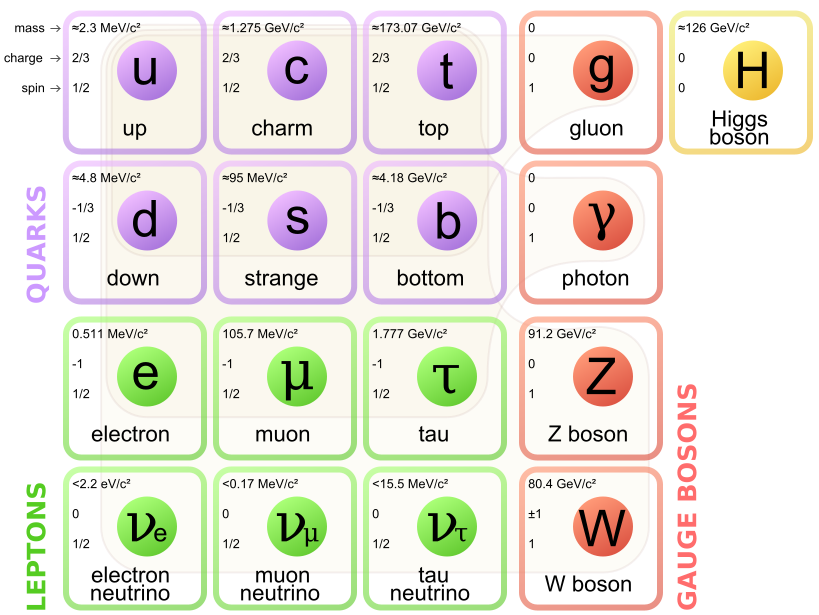
\includegraphics[width=\textwidth]{figures/Standard_Model_of_Elementary_Particles.png}
      \end{figure}
    \end{center}
\end{frame}

\begin{frame}{The Standard Model Circa 1973}
  \begin{itemize}
    \item Only discovered quarks were up, down, and strange
    \pause\
    \item Parity and charge have been discovered to be independently violated in
      \begin{equation*}
        \pi^{+} \rightarrow \mu^{+}+\nu_{\mu}
      \end{equation*}
    \pause\
    \item So $CP$ was proposed as the ``real'' mirror symmetry
    \pause\
    \item $CP$ violation led to the proposal of a third generation of quarks
  \end{itemize}
\end{frame}

\begin{frame}{The Neutral Kaon}
  \begin{columns}
    \begin{column}{0.5\textwidth}
      \begin{itemize}
        \item $K^0$ are produced via strong interactions with definite quark flavour content.
        \pause\
        \item However, certain diagrams allow for $K^0\rightleftharpoons\overbar{K^0}$ mixing
        \pause\
        \item The result is that Kaons evolve into superpositions of $K^0$ and $\overbar{K^0}$
      \end{itemize}
    \end{column}
    \begin{column}{0.5\textwidth}
      \begin{center}
        \begin{figure}
          \includegraphics<2->[width=\textwidth]{figures/Kaon_Mixing}
        \end{figure}
      \end{center}
    \end{column}
  \end{columns}
\end{frame}

\begin{frame}{The Neutral Kaon \-- $CP$ Eigenstates}
  \begin{itemize}
  \item The action of $C$,$P$, and $CP$ on the $\ket{K^0},\ket{\overbar{K^0}}$ system:
    \begin{align*}
      \pause\
      C\ket{K^0}=\ket{\overbar{K^0}} \quad&\quad C\ket{\overbar{K^0}}=\ket{K^0} \\
      \pause\
      P\ket{K^0}=-\ket{K^0} \quad&\quad P\ket{\overbar{K^0}}=-\ket{\overbar{K^0}} \\
      \pause\
      CP\ket{K^0}=-\ket{\overbar{K^0}} \quad&\quad CP\ket{\overbar{K^0}}=-\ket{K^0}
    \end{align*}
  \item Two eigenstates of $CP$ can be formed.
    \begin{equation*}
      \ket{K_1}=\frac{1}{\sqrt{2}}\left(\ket{K^0}-\ket{\overbar{K^0}}\right) ,\quad \ket{K_2}=\frac{1}{\sqrt{2}}\left(\ket{K^0}+\ket{\overbar{K^0}}\right)
    \end{equation*}
  \end{itemize}
\end{frame}

\begin{frame}{The Neutral Kaon \-- Allowed Decays}
  \begin{itemize}
    \item If the weak interaction conserves $CP$, then $\ket{K_1}$ can only decay into states with $CP=1$ and $\ket{K_2}$ only to states with $CP=-1$.
    \pause\
  \item For example,
    \begin{columns}
      \begin{column}{0.5\textwidth}
      \begin{align*}
        \quad \quad \quad \quad \quad \quad \quad \quad K_1 \rightarrow& 2\pi \\
        K_2 \rightarrow& 3\pi
      \end{align*}
      \end{column}
      \begin{column}{0.5\textwidth}
        \vfill
        \color{green}{Allowed}
      \end{column}
    \end{columns}
    \begin{columns}
      \begin{column}{0.5\textwidth}
      \begin{align*}
        \quad \quad \quad \quad \quad \quad \quad \quad K_1 \rightarrow& 3\pi \\
        K_2 \rightarrow& 2\pi
      \end{align*}
      \end{column}
      \begin{column}{0.5\textwidth}
        \vfill
        \color{red}{Forbidden}
      \end{column}
    \end{columns}
  \end{itemize}
\end{frame}

\begin{frame}{The Neutral Kaon \-- $CP$ Violation}
  \begin{itemize}
    \item Furthermore, since the $K_1 \rightarrow 2\pi$ process happens much more quickly, the $K_1$ component of the superposition
      \begin{equation*}
        \ket{\Psi} = \alpha\ket{K_1} + \beta\ket{K_2}
      \end{equation*}
      quickly disappears, leaving only
      \begin{equation*}
        \ket{\Psi} = \ket{K_2}
      \end{equation*}
      \pause\
    \item So a beam of neutral kaons consists of only a tiny fraction of $K_1$ after a few meters.
    \pause\
  \item If the ``forbidden'' process $K_2 \rightarrow 2\pi$ is observed down the beamline, it means that $CP$ is not a true symmetry.
  \end{itemize}
\end{frame}

\begin{frame}{$CP$ Violation}
  \begin{itemize}
    \item $CP$ Violation posed a theoretical problem with only two quark generations.
    \pause\
    \item The weak eigenstates of the down type quarkes are related to the flavor eigenstates via the Cabibbo angle $\theta_C$.
      \begin{equation*}
        \begin{pmatrix} d' \\ s' \end{pmatrix} =
        \begin{pmatrix}
          \cos\theta_C & \sin\theta_C \\
          -\sin\theta_C & \cos\theta_C \\
        \end{pmatrix}
        \begin{pmatrix} d \\ s \end{pmatrix}
      \end{equation*}
    \pause\
    \item But because the matrix elements are strictly real, $CP$ is still conserved.
  \end{itemize}
\end{frame}

\begin{frame}{$CP$ Violation}
  \begin{itemize}
    \item However, with three quark generations there is instead this relation
      \begin{center}
      {\tiny
      \begin{equation*}
        \begin{pmatrix} d' \\ s' \\ b' \end{pmatrix} =
        \begin{pmatrix}
          c_{12}c_{13}                                  & s_{12}c_{13}                               & s_{13}e^{-i\delta} \\
          -s_{12}c_{23}-c_{12}s_{23}s_{13}e^{i\delta}   & c_{12}c_{23} - s_{12}s_{23}s_{13}e^{i\delta} & s_{23}c_{13} \\
          s_{12}c_{23}-c_{12}s_{23}s_{13}e^{i\delta}    & -c_{12}c_{23} - s_{12}s_{23}s_{13}e^{i\delta} & c_{23}c_{13} \\
        \end{pmatrix}
        \begin{pmatrix} d \\ s \\ b \end{pmatrix}
      \end{equation*}
      }
      \end{center}
      \pause\
    \item Notice that the presence of $\delta$ means that some elements are necessarily complex, allowing for $CP$ violation.
    \pause\
    \item This motivated the prediction of a third quark generation. (Note that this was even before the discovery of the charm)
  \end{itemize}
\end{frame}

\begin{frame}{$CP$ Violation \-- Mechanism}
  \begin{figure}
    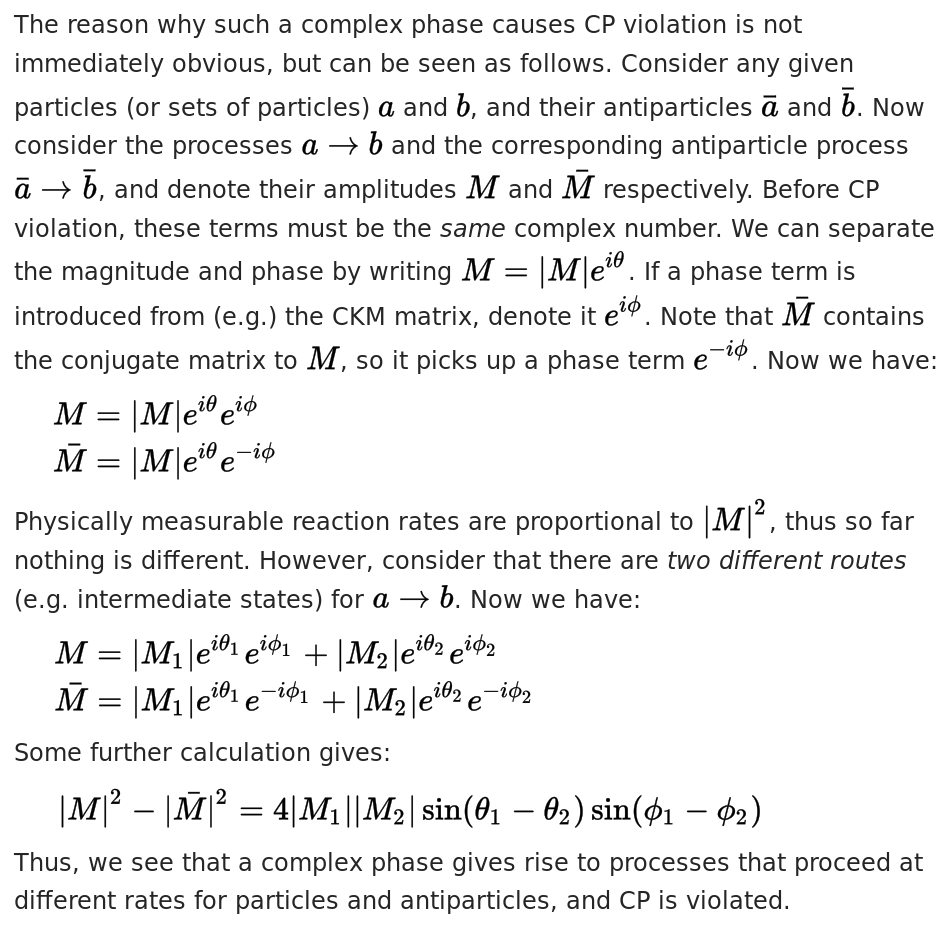
\includegraphics[height=0.9\textheight]{figures/CP_Violation_Explain.png}
  \end{figure}
\end{frame}

\begin{frame}{Bottom Quark Discovery \-- 1977}
  \begin{figure}
    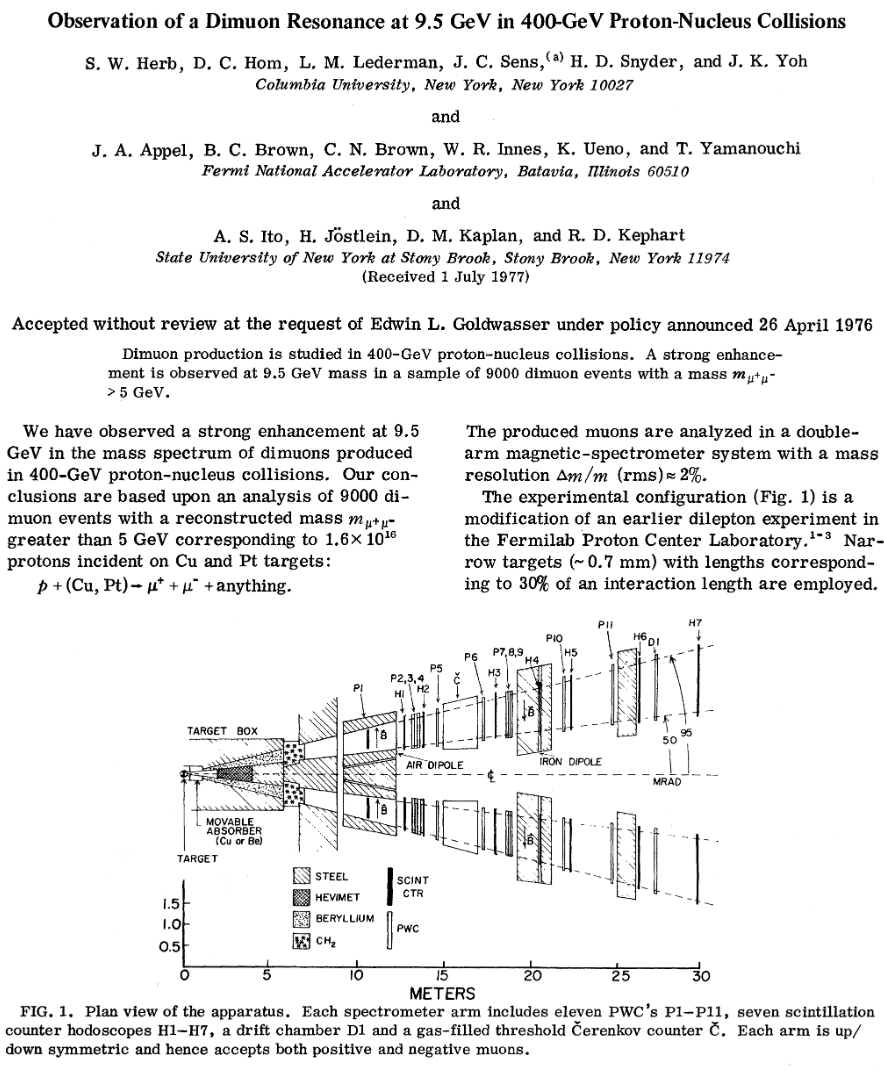
\includegraphics[height=0.9\textheight]{figures/Bottom_Quark_Discovery.png}
  \end{figure}
\end{frame}

\begin{frame}{Top Quark Discovery \-- 1995}
  \begin{figure}
    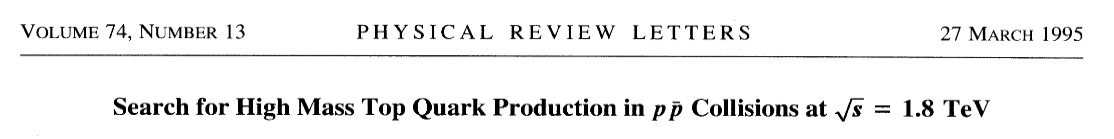
\includegraphics[width=\textwidth]{figures/Top_Quark_Discovery_1.png}
  \end{figure}
  \hrule
  \begin{figure}
    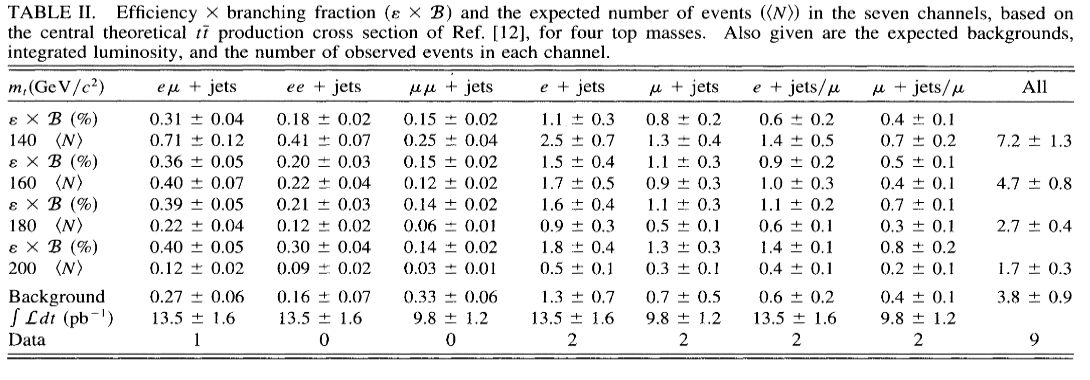
\includegraphics[width=\textwidth]{figures/Top_Quark_Discovery_2.png}
  \end{figure}
\end{frame}

\begin{frame}{Top Quark Production at LHC}
  \begin{columns}
    \begin{column}{0.3\textwidth}
      Some common top quark production modes
    \end{column}
    \begin{column}{0.7\textwidth}
      \begin{figure}
        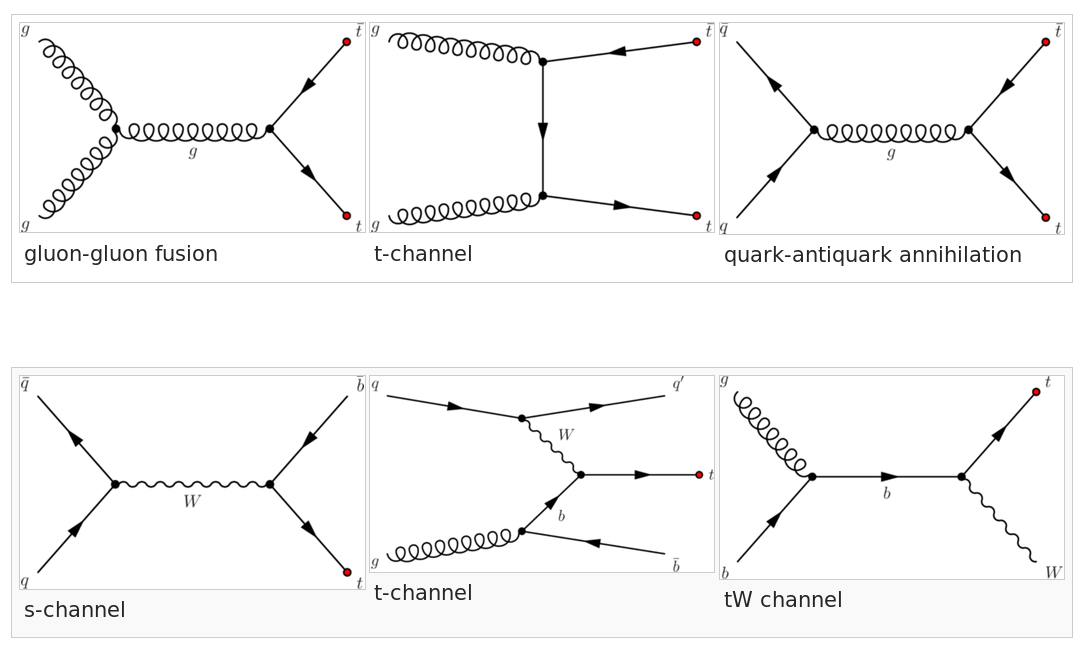
\includegraphics[height=0.45\textheight]{figures/Top_Quark_Production.png}
      \end{figure}
    \end{column}
  \end{columns}
  \pause\
  \hrule
  \begin{columns}
    \begin{column}{0.4\textwidth}
      ``Parton Distribution Function'' for a proton at $Q=2\si{\giga\electronvolt}$
    \end{column}
    \begin{column}{0.6\textwidth}
      \begin{figure}
        \includegraphics<2->[height=0.40\textheight]{figures/Parton_Distribution_Functions.png}
      \end{figure}
    \end{column}
  \end{columns}
\end{frame}

\begin{frame}{Top Quark Decay}
  \centering
  \includegraphics<1>[width=0.80\textwidth]{figures/Top_antitop_quark_event.png}
  \includegraphics<2>[width=0.60\textwidth]{figures/Top_antitop_quark_event.png}
  \pause\
  \hrule
  Possible Final States
  \begin{itemize}
    \item $2\text{ B-Jets } + 4\text{ ``light'' Jets }$
    \item $2\text{ B-Jets } + 2\text{ ``light'' Jets } + 1\text{ lepton } + 1\text{ neutrino }$
    \item $2\text{ B-Jets } + 2\text{ leptons } + 2\text{ neutrinos }$
  \end{itemize}
\end{frame}

% \begin{frame}{References}
%     % \nocite{*}
%     \bibliographystyle{abbrv}
%     {\tiny
%     \bibliography{references}
%     }
% \end{frame}

\end{document}
